\chapter{Time-dependent Edge Cost Estimation}
Chapter~\ref{Ch:ldmk_graph} describes the general procedures for constructing a landmark graph. To find a time-dependent shortest route on a landmark graph, the time-dependent edge cost must be calculated. In this project, the time-dependent edge cost specifically refers to travel time, but in theory, it can refer to any quantity that can be described as a time-dependent edge cost function of the form $w : E,t \rightarrow \mathbb{R}$. In practice, it sometimes also refers to fuel consumptions or taxi fares. This chapter introduces a machine learning-based approach to estimate the travel time of each \emph{significant edge} in a landmark graph at a particular moment in time. 

\begin{defn}[\emph{Significant Edge}]
A significant edge in a landmark graph $G=(V,E)$ is an edge $e \in E$ that appears at least $m$ times, where $m$ is a parameter specified in advance.
\end{defn}

The purpose of defining significant edges is to eliminate those edges that are seldom traversed by taxi drivers, as estimating the travel time of those edges will not be very accurate. The parameter $m$ also represents a level of \emph{confidence}\footnote{Sometimes it is also referred to as \emph{support}}, that is, to what extent it is true that this edge \emph{really} exists in the real world. 

Everyday experiences show that the travel time of a particular road usually has different time-varying patterns in weekdays as compared to that in weekends or public holidays. For instance, it is likely that, on weekdays, the travel time of a particular road has one \emph{peak} at 8 a.m. when people travel to work and the other peak at 6 p.m. when people return home after work. But when it is weekends or public holidays, the travel time of that road may have a peak at 10 a.m. when people go for holiday activities with families and the other peak at only about 8 p.m. when the whole day's celebrations are over. 

Based on this intuition, two separate landmark graphs were built in this project, with one for weekdays and the other for weekends or public holidays. Moreover, as mentioned in Section~\ref{Subsec:outlier_removal}, 
two data sets, bjtaxigps\_30m and bjtaxigps\_50m, remained after outlier removal based on different thresholds set for removing outliers. Therefore, in total, \emph{four} landmark graphs were built in this project and they are summarised in Table~\ref{Ta:ldmkgraphs}, although their names are self-explanatory. 

\begin{table}[h!]
\centering
\resizebox{\columnwidth}{!}{
\begin{tabular}{ | c | c | }
\hline
\textbf{Landmark Graph} & \textbf{Data Source} \\ \hline
wrkd\_ldmkgraph\_30m & weekday trajectories in bjtaxigps\_30m\\\hline
holi\_ldmkgraph\_30m & holiday trajectories in bjtaxigps\_30m \\\hline
wrkd\_ldmkgraph\_50m & weekday trajectories in bjtaxigps\_50m\\\hline
holi\_ldmkgraph\_50m  & holiday trajectories in bjtaxigps\_50m\\ \hline
\end{tabular}}
\caption{An summary of landmark graphs}\label{Ta:ldmkgraphs}
\end{table}

\section{Travel Time Distribution}
\begin{figure}[h!]
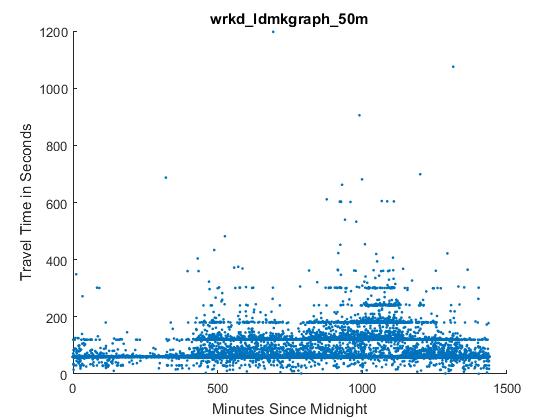
\includegraphics[scale=0.85]{trvltime_scatter}
\centering
\caption{An example of travel time patterns}\label{Fig:wrkd_50m_trvltime}
\end{figure}

Figure~\ref{Fig:wrkd_50m_trvltime} illustrates a scatter plot of the travel time of a particular landmark graph edge during the course of a weekday. It can be observed that the travel time does not seem to be a single-valued function with respect to time of the day, as one may expect; rather, the scatter points tend to gather around some values and form some \emph{clusters}. For instance, when it is 500 minutes since midnight, namely 8:20~a.m., the travel time seems to have three main clusters which are represented by three horizontal lines formed by the scatter points. When it is 1,000 minutes since midnight, namely 4:40~p.m., there are about five such lines. This pattern is attributable to three possible reasons:
\begin{enumerate}
\item Drivers may actually choose different routes to travel between the two landmarks, which cannot be captured by the landmark graph since it only knows a driver has traversed between the two landmarks but not the exact route. Different routes have different traffic conditions and speed limitations, therefore the travel time varies;
\item Drivers have different driving skills, preferences and behaviours. Some drivers just drive faster than others, even if the road conditions are similar and;
\item The GPS devices on taxis reported locations \emph{periodically}, therefore, durations like 60 secondsr or120 seconds are very commonly seen in the landmark graphs. Even if the \emph{actual} travel time is 53 seconds, it is still recorded as 60 seconds. This corresponds to the low-sampling-rate problem mentioned in Section~\ref{Sec:limitation}. 
\end{enumerate}

\begin{figure}[h!]
\centering
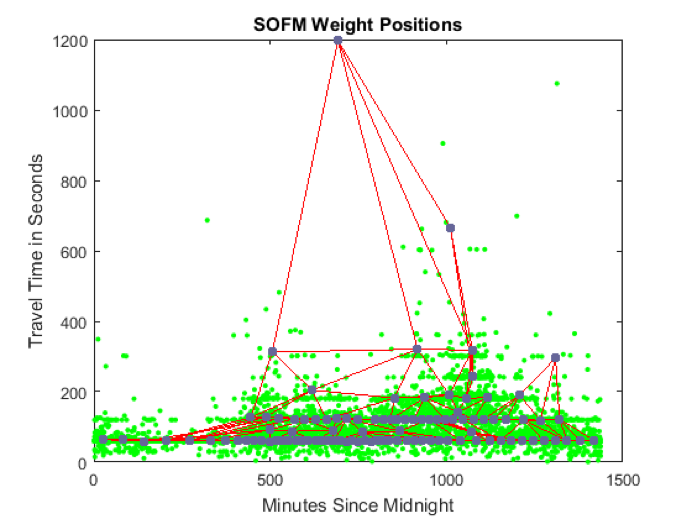
\includegraphics[scale=0.85]{trvltime_clus} 
\caption{Final positions of the neurons}\label{Fig:trvltime_clus}
\end{figure}

Therefore, it is not possible to fit the scatter points with a single-valued function. Rather, the clustering technique should first be employed to identify the travel time clusters. Like in Section~\ref{SubSec:outlier_identify}, a \textbf{self-organising feature map} is used to cluster the scatter points. Figure~\ref{Fig:trvltime_clus} shows the final positions of the neurons at the end of the training.

\begin{figure}[h!]
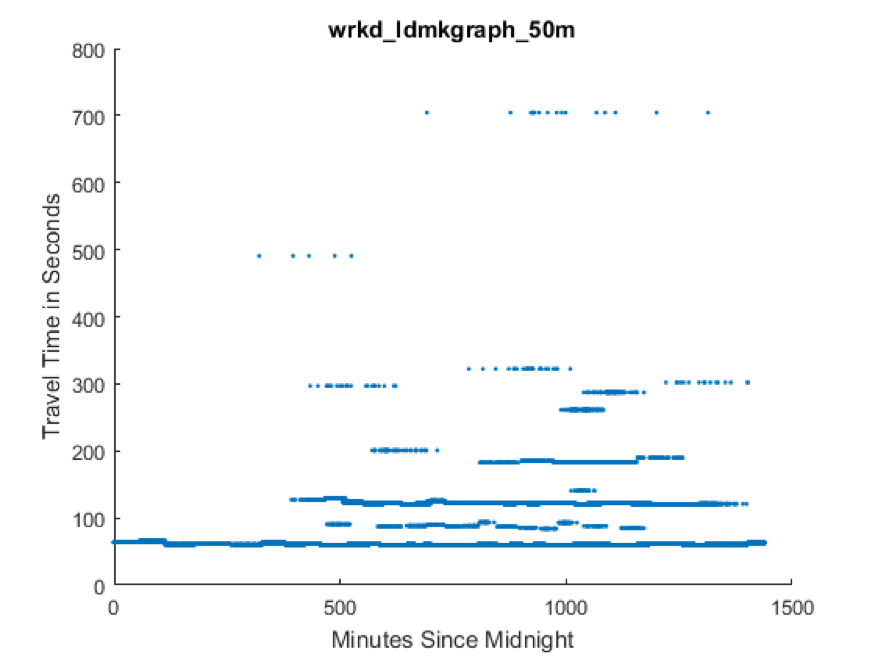
\includegraphics[scale=0.85]{trvltime_neurons}
\centering
\caption{An example of representing data points with centroids}\label{Fig:trvltime_neurons}
\end{figure}

One merit of SOFM clustering is \emph{feature extraction}. In this case, after the training is completed, the SOFM has learned some features about the travel time at different time of the day and expressed its understanding by moving its neurons to the centroids of the clusters. Now, \textbf{the data points can be represented by their respective centroids}. Figure~\ref{Fig:trvltime_neurons} shows the effect of replacing each data point's value with their centroids'. The clusters are clearly shown by the horizontal lines formed by those centroids. 

Now that the clusters are identified, the next step is \textbf{to estimate the distributions of clusters within a specific time interval}. This is based on the assumption that within that interval the travel time patterns do not change; therefore, a distribution of clusters can be used to describe the pattern in that interval. In this project, an interval of 30 minutes was used. Figure~\ref{Fig:clus_histo} shows an example of a distribution of clusters within 10:00~a.m. to 10:30~a.m. interval.

\begin{figure}[h!]
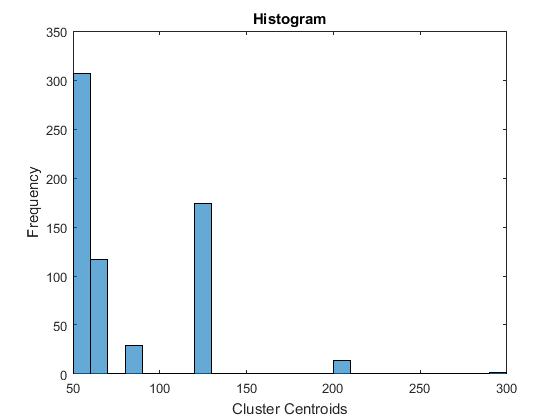
\includegraphics{clus_histo}
\centering
\caption{An example of distribution of clusters}\label{Fig:clus_histo}
\end{figure}

The distribution of clusters is then converted into a cumulative distribution